\section{Aplicación de la Metodología XP}
\subsection{Exploración}
Antes de especificar las historias de usuario, fue necesario asignar los roles de cada uno de los participantes del proyecto. De manera que quedaron así: 

\begin{itemize}
    \item \textbf{Desarrollador:} Sebastián y Natalia (los autores).
    \item \textbf{Cliente: } Institución Educativa Juan María Céspedes.
    \item \textbf{Tracker: } Iván Eduardo Gálvez Giraldo (docente de la asignatura de Física del grado Décimo).
    \item \textbf{Manager: }Carlos Andrés Delgado Saavedra (director de trabajo de grado).
\end{itemize}

\subsubsection{Historias de Usuario}
El Cliente, en este caso el docente de física Iván Eduardo Gálvez Giraldo, en representación de la Institución Educativa Juan María Céspedes sugirió las características que el sistema debía tener, aunque en la Metodología XP, el cliente es el encargado de realizar las historias de usuario, fueron los desarrolladores que convirtieron estas características sugeridas por el cliente en Historias de usuario. 

En total, se obtuvieron 31 Historias de Usuarios, las cuales representaban los requisitos que debía tener la aplicación. Cada historia de usuario fue estimada utilizando la secuencia de Fibonacci (1, 2, 3, 5, 8, 13, 21), es decir, a cada historia de usuario se le asignó uno de los números de esta secuencia.

Así pues, una historia de usuario asignada con estimación de 2, requerirá el doble de esfuerzo que una estimada con 1 y una que esté estimada con 3, requerirá el triple de esfuerzo que una estimada en 1 y así sucesivamente.

A continuación, se muestra algunas historias de usuario:

\begin{figure}[H]
\begin{tabular}{|p{3.5cm}|p{3.5cm}|p{4cm}|p{4cm}|}
\hline
\multicolumn{4}{|>{\columncolor[rgb]{0.9,0.9,0.9}}l|}{ \textbf{Historia de Usuario}}\\
\hline
\multicolumn{1}{|p{3cm}|}{\textbf{No.} 1 }&\multicolumn{3}{|p{12cm}|}{\textbf{Usuario: } Estudiante}\\
\hline
\multicolumn{2}{|p{7cm}|}{\textbf{Nombre Historia: } Registrar Estudiante  }&\multicolumn{2}{|p{8cm}|}{\textbf{Responsable: }Natalia Rubiano Silva }\\
\hline
\textbf{Prioridad: }Alta&\multicolumn{2}{|p{7.5cm}|}{ \textbf{Puntos Estimados: }3}&\textbf{Iteración: }1\\
\hline
\multicolumn{4}{|p{15cm}|}{ \textbf{Descripción: }}\\
\multicolumn{4}{|p{15cm}|}{ Como un usuario estudiante necesito registrarme al sistema con el objetivo de poder acceder a las funcionalidades e interactuar con el.}\\
\hline
\multicolumn{4}{|p{15cm}|}{ \textbf{Observación: }}\\
\multicolumn{4}{|p{15cm}|}{ No hay observaciones.}\\
\hline
\end{tabular}
    \caption{Historia de Usuario Nº1}
    \centering \scriptsize \textbf{Fuente:} Elaboración propia
\end{figure}

\begin{figure}[H]
\begin{tabular}{|p{3.5cm}|p{3.5cm}|p{4cm}|p{4cm}|}
\hline
\multicolumn{4}{|>{\columncolor[rgb]{0.9,0.9,0.9}}l|}{ \textbf{Historia de Usuario}}\\
\hline
\multicolumn{1}{|p{3cm}|}{\textbf{No.} 2 }&\multicolumn{3}{|p{12cm}|}{\textbf{Usuario: } Administrador}\\
\hline
\multicolumn{2}{|p{7cm}|}{\textbf{Nombre Historia: } Registrar Docente  }&\multicolumn{2}{|p{8cm}|}{\textbf{Responsable: }Johan Sebastián Cárdenas Sánchez }\\
\hline
\textbf{Prioridad: }Alta&\multicolumn{2}{|p{7.5cm}|}{ \textbf{Puntos Estimados: }3}&\textbf{Iteración: }2\\
\hline
\multicolumn{4}{|p{15cm}|}{ \textbf{Descripción: }}\\
\multicolumn{4}{|p{15cm}|}{ Como un usuario administrador necesito registrar a los usuarios docentes que harán uso del sistema con el objetivo de que estos puedan acceder a las funcionalidades e interactuar con ella.}\\
\hline
\multicolumn{4}{|p{15cm}|}{ \textbf{Observación: }}\\
\multicolumn{4}{|p{15cm}|}{Estar logueado al sistema.}\\
\hline
\end{tabular}
    \caption{Historia de Usuario Nº2}
    \centering \scriptsize \textbf{Fuente:} Elaboración propia
\end{figure}

El resto de las Historias de Usuarios se encuentran en:  \textbf{(Carpeta Anexos, documento: Historias de Usuario)}.

\subsubsection{Usuarios del Sistema y Roles}
Con base en el análisis de las Historia de Usuario se determinaron los roles que el sistema debía tener.  En la siguiente tabla se muestran la definición y funciones de dichos roles:

\begin{table}[H]
    \centering
    \begin{tabular}{|p{3cm}|p{12cm}|}
        \hline
        \textbf{Rol} & \textbf{Funciones} \\
        \hline
        & Acceder al contenido de la aplicación desde el monitor para llevar a cabo el proceso de aprendizaje pertinente. \\
        Estudiante& Desarrollar cuestionarios planteados acerca de los temas de la cinemática.\\
        & Consultar el progreso de los temas.\\
       \hline
        & Acceder al contenido de la aplicación web desde el monitor. \\
        Docente& Establecer las preguntas y respuestas que deben tener los cuestionarios.\\
        & Consultar las calificaciones de los estudiantes de los cuestionarios previamente diligenciados.\\
        & Habilitar y deshabilitar el usuario estudiantes.\\
        \hline
        & Registrar a los estudiantes, docentes. \\
        Administrador& Registrar las preguntas y respuestas de los cuestionarios.\\
        & Consultar los estudiantes, docentes y cuestionarios pertenecientes a la aplicación.\\
       \hline
    \end{tabular}
    \caption{Usuarios del Sistema}
    \centering \scriptsize \textbf{Fuente:} Elaboración propia
    \label{tab:usSis}
\end{table}

\subsubsection{Definición de tecnologías }
Con las historias de usuario planteados del proyecto, se definieron qué tecnologías se iban a utilizar para el desarrollo de este. 


Teniendo en cuenta, la gran cantidad de tecnología para el desarrollo del FrontEnd y del BackEnd de un proyecto, se realizó una revisión de las tecnologías de cada una de ellas, con el fin de elegir la más adecuada para el presente proyecto. \ \\

\textbf{Herramientas del Frontend: }Para el desarrollo del FrontEnd se analizó Bootstrap y Foundation, las cuales permiten la creación de interfaces web con CSS y JavaScript. Estas  facilitan la codificación, y permiten adaptar la interfaz del sitio web al tamaño del dispositivo que se visualice. A continuación, se muestra un cuadro comparativo de estas dos tecnologías:

\begin{table}[H]
    \centering
    \begin{tabular}{|p{3cm}|p{6cm}|p{6cm}|}
        \hline
        \textbf{Características}&\textbf{Bootstrap}&\textbf{Foundation}\\
        \hline
        \textbf{Personalización}&Al tener componentes bien pulidos y listos para usar permite crear un sitio web rápido, sin embargo, el estilo de estos componentes se puede anular.& Puede llevar mucho tiempo personalizar un sitio web. \\
        \hline
         \multicolumn{1}{|p{3cm}|}{ \textbf{Soporte del navegador}}&\multicolumn{2}{|p{12cm}|}{Ofrecen un excelente soporte de navegador para las últimas versiones de los principales navegadores: Chrome, Safari, Firefox, Opera.}\\
        \hline
        \textbf{Sistema de red}&Sistema de cuadrícula que soporta 12 columnas.&Sistema de cuadrícula que soporta 12 columnas, con diseño flexible. \\
        \hline
        \textbf{Documentación}&Muy elaborada y explicativa.&No es tan clara y organizada en comparación con Bootstrap. \\
        \hline
        \textbf{Cantidad de recursos}&Gran cantidad de plantillas, temas, complementos de terceros.&Una serie de plantillas, temas, complementos de terceros.. \\
        \hline
        \textbf{Popularidad}&El más popular entre todos los marcos FrontEnd.&No es tan popular en comparación con Bootstrap.\\
        \hline
        \textbf{Comunidad}&Tiene la comunidad en línea más grande entre los marcos FrontEnd.&Tiene una comunidad más pequeña, pero en constante crecimiento.\\
        \hline
    \end{tabular}
    \caption{Comparación de herramientas FrontEnd}
    \centering \scriptsize \textbf{Fuente:} Elaboración propia
    \label{tab:frontEnd}
\end{table}

Pese a que ambas tecnologías tienen grandes fortalezas y son de gran ayuda para el desarrollo del FrontEnd, se determinó que Bootstrap sería la elegida debido a su fácil entendimiento en la documentación y también por la gran comunidad que tiene ya que facilita cualquier tipo de consulta y permite resolver cualquier duda que se tenga. \ \\

\textbf{Herramientas del BackEnd: }En cuanto al desarrollo del BackEnd, se ha tenido en cuenta las limitaciones de la infraestructura del colegio, por lo tanto, se escoge como lenguaje de programación PHP. En la tabla \ref{tab:backEnd}, se analizaron los frameworks  Laravel y Symfony.

\begin{table}[H]
    \centering
    \begin{tabular}{|p{3cm}|p{6cm}|p{6cm}|}
        \hline
        \textbf{Características}&\textbf{Laravel}&\textbf{Symfony}\\
        \hline
         \textbf{Plantillas}&Uso de blade que permite la reutilización de código.&Uso de Twig, donde es necesario definir una misma función dos veces. \\
        \hline
        \textbf{Arquitectura}&MVC&MVC \\
        \hline
        \textbf{Velocidad de desarrollo}&Desarrollo rápido.&Menos rápido que laravel.\\
        \hline
        \multicolumn{1}{|p{3cm}|}{ \textbf{Escalabilidad}}&\multicolumn{2}{|p{12cm}|}{Permiten la escalabilidad.}\\
        \hline
        \textbf{Mapeo de objetos}&Propia biblioteca Eloquent.&Usa proyecto de terceros “Doctrine” para interactuar con la base de datos.\\
        \hline
        \textbf{Documentación}&Gran cantidad de tutoriales y vídeos de soporte&Básica.\\
        \hline
    \end{tabular}
    \caption{Comparación de herramientas BackEnd}
    \centering \scriptsize \textbf{Fuente:} Elaboración propia
    \label{tab:backEnd}
\end{table}

Ahora bien, pese a que los dos framework soportan escalabilidad, el framework elegido fue Laravel, principalmente porque permite un desarrollo más rápido, tiene gran cantidad de documentación y además su código es intuitivo siendo así que sea amigable para el desarrollador.

\subsubsection{Arquitectura del sistema}
Con la selección de tecnologías se estableció la arquitectura general del sistema, la cual se basa en un modelo cliente-servidor, orientada en tres capas: modelo, vista y controlador. Tal como se muestra en la siguiente figura.

\begin{figure}[H]
    \centering
    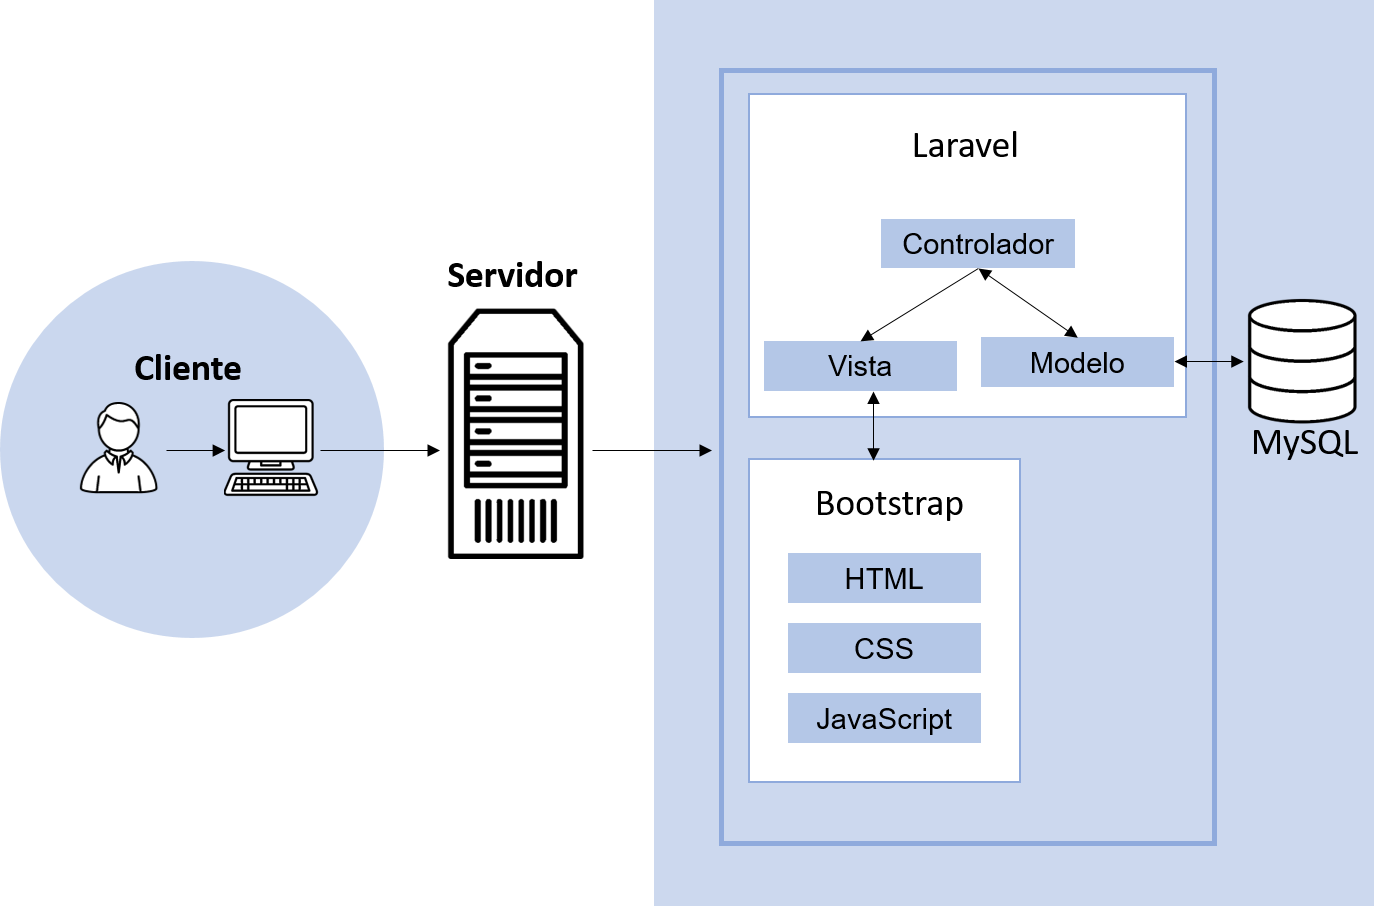
\includegraphics[scale=0.4]{Capitulo_4/2_XP/imagenes/arquitecturaSistema.png}
    \caption{Arquitectura del Sistema}
    \scriptsize \textbf{Fuente:} Elaboración propia
    \label{fig:arquitectura}
\end{figure}

La capa modelo es la encargada de los datos, es decir, es la que accede a la información; por su parte, la capa vista es la interfaz de usuario que permite presentar los datos que el modelo proporciona; mientras que la capa controlador es el enlace entre la capa modelo y vista, es el encargado de la lógica, controla las entradas y salidas de información, responde a los eventos y acciones que pasan.

\textbf{Funcionamiento de la arquitectura: } El cliente solicita una petición, la petición se redirecciona al controlador, este responde la solicitud y a continuación le solicita a la capa modelo la información necesaria. La capa modelo, consulta la base de datos y obtiene lo que solicita y responde a la capa controlador con los datos solicitados, cuando la capa controlador tiene los datos solicitados, los envía a la capa vista y esta organiza la información con los estilos correspondientes y finalmente se muestra al cliente.

\subsubsection{Modelo Entidad - Relación}
\begin{figure}[H]
    \centering
    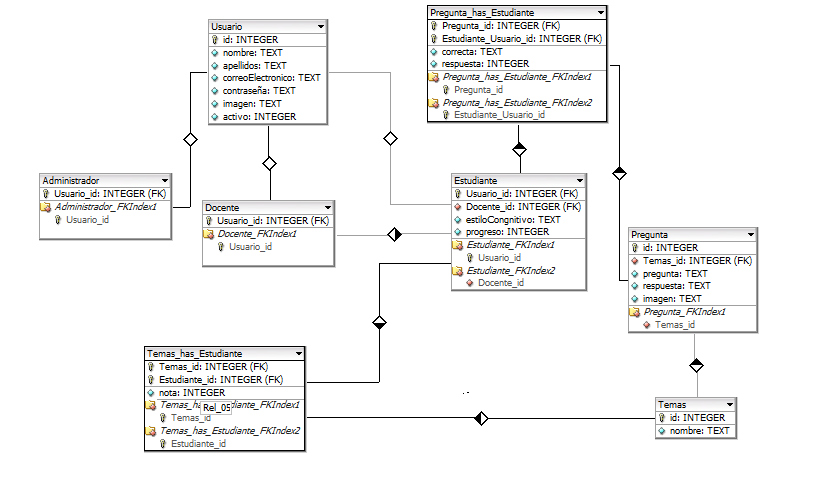
\includegraphics[scale=0.7]{Capitulo_4/2_XP/imagenes/mer.png}
     \caption{Modelo Entidad - Relación}
    \scriptsize \textbf{Fuente:} Elaboración propia
    \label{fig:MER}
\end{figure}
En la figura \ref{fig:MER} se muestra el modelo de entidad relación de la base de datos donde se almacenaron los datos utilizados en la aplicación.

A continuación, se explica las entidades que los componen:

\begin{itemize}
    \item Entidad usuario, donde un usuario puede ser un administrador, un docente o un estudiante. 

    \item Entidad tema, en donde se almacenan las unidades de aprendizaje de la aplicación y posee una relación de uno a muchos, con otra entidad llamada preguntas.
    
    Asimismo, esta entidad una relación de muchos a muchos con la entidad estudiante ya que un tema lo ven muchos estudiantes y un estudiante puede ver varios temas

    \item Entidad pregunta tiene una relación de muchos a muchos con la entidad estudiante ya que un estudiante puede resolver muchas preguntas y una pregunta puede ser resuelta por muchos estudiantes.
\end{itemize}


\subsubsection{Prototipos de Interfaces }
Los prototipos sirven para hacer un boceto de cómo será la interfaz de la aplicación y muestran el modo de interactuar los usuarios con ella. A continuación, se muestran los prototipos que se realizaron para el sistema:

\begin{figure}[H]
    \centering
    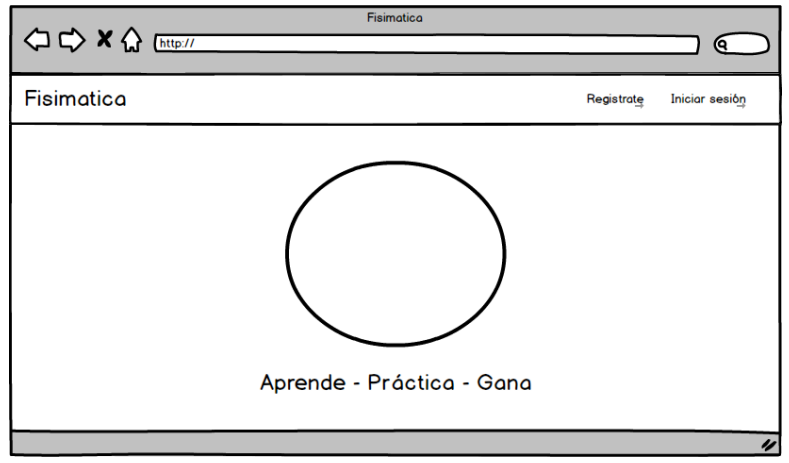
\includegraphics[scale=0.4]{Capitulo_4/2_XP/imagenes/inicial.png}
     \caption{Prototipo de la pantalla inicial}
    \scriptsize \textbf{Fuente:} Elaboración propia
    \label{fig:PInicial}
\end{figure}

\begin{figure}[H]
    \centering
    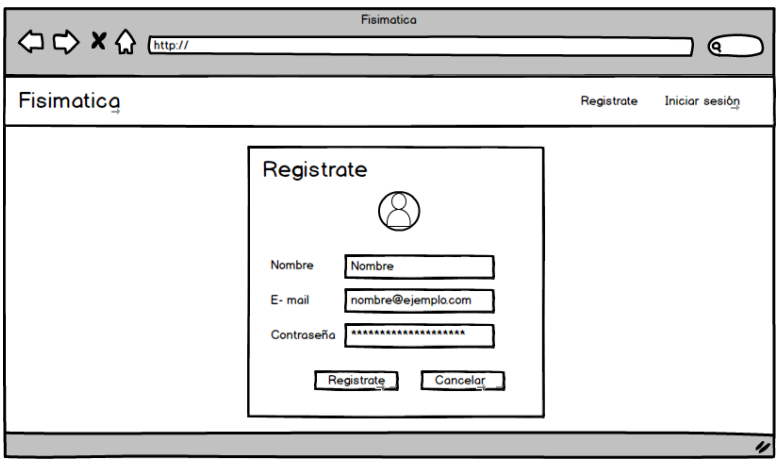
\includegraphics[scale=0.4]{Capitulo_4/2_XP/imagenes/registro.png}
     \caption{Prototipo de la pantalla de registro}
    \scriptsize \textbf{Fuente:} Elaboración propia
    \label{fig:PRegistro}
\end{figure}
Para las dos categorías de estilos cognitivos que el sistema se va adaptar se crearon los siguientes prototipos:


\begin{itemize}
    \item \textbf{Categoría Independiente del Campo}\\
    En el caso de la categoría independiente del campo, se ofrece un menú donde el alumno puede optar por realizar los temas de aprendizaje en cualquier orden.
    \begin{figure}[H]
        \centering
        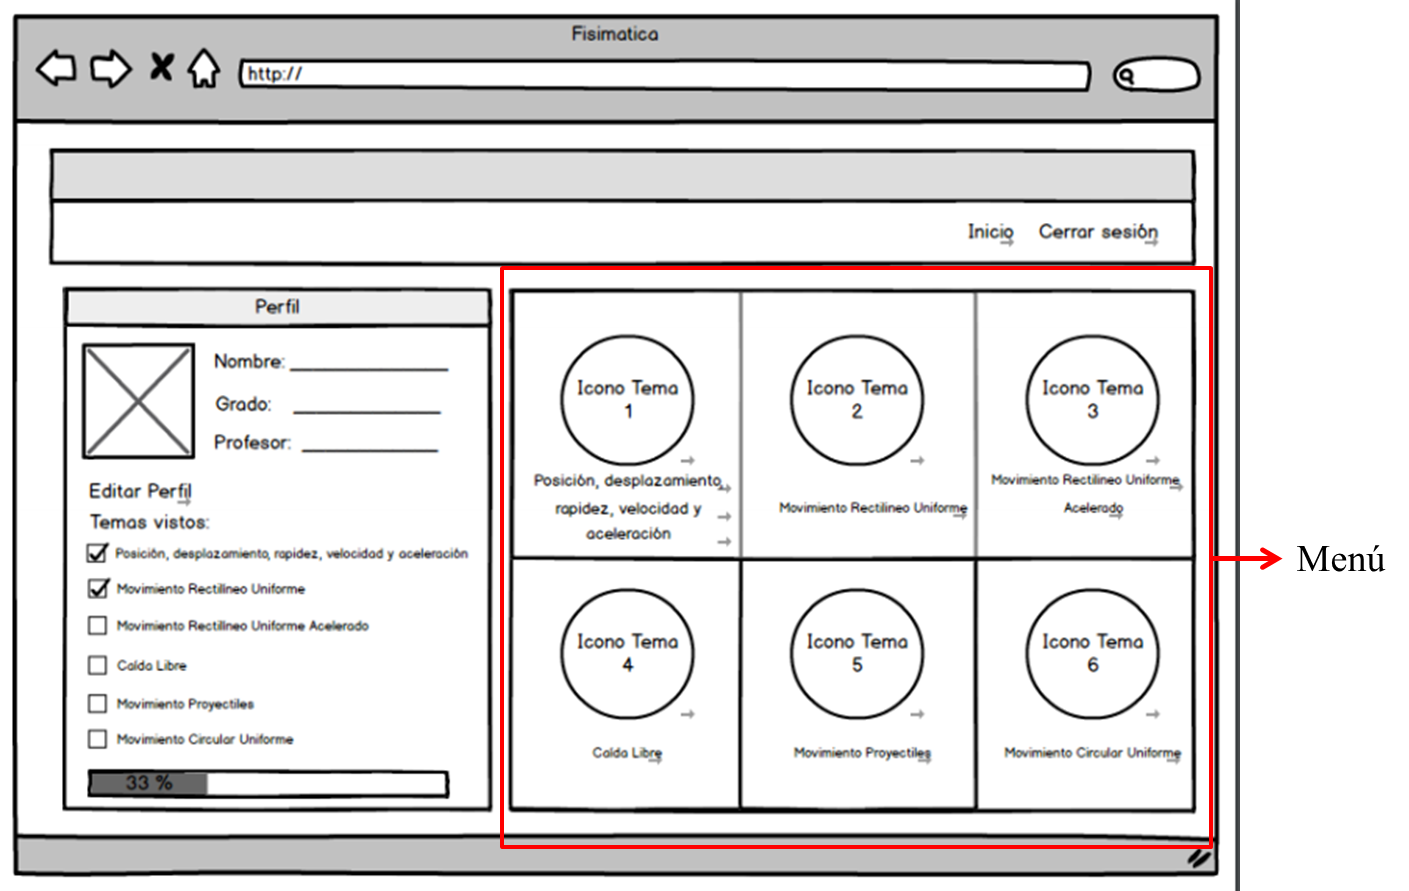
\includegraphics[scale=0.4]{Capitulo_4/2_XP/imagenes/navLibre.png}
         \caption{Prototipo de navegación Libre - Menú Inicial}
        \scriptsize \textbf{Fuente:} Elaboración propia
        \label{fig:navLibre}
    \end{figure}
    
    \begin{figure}[H]
        \centering
        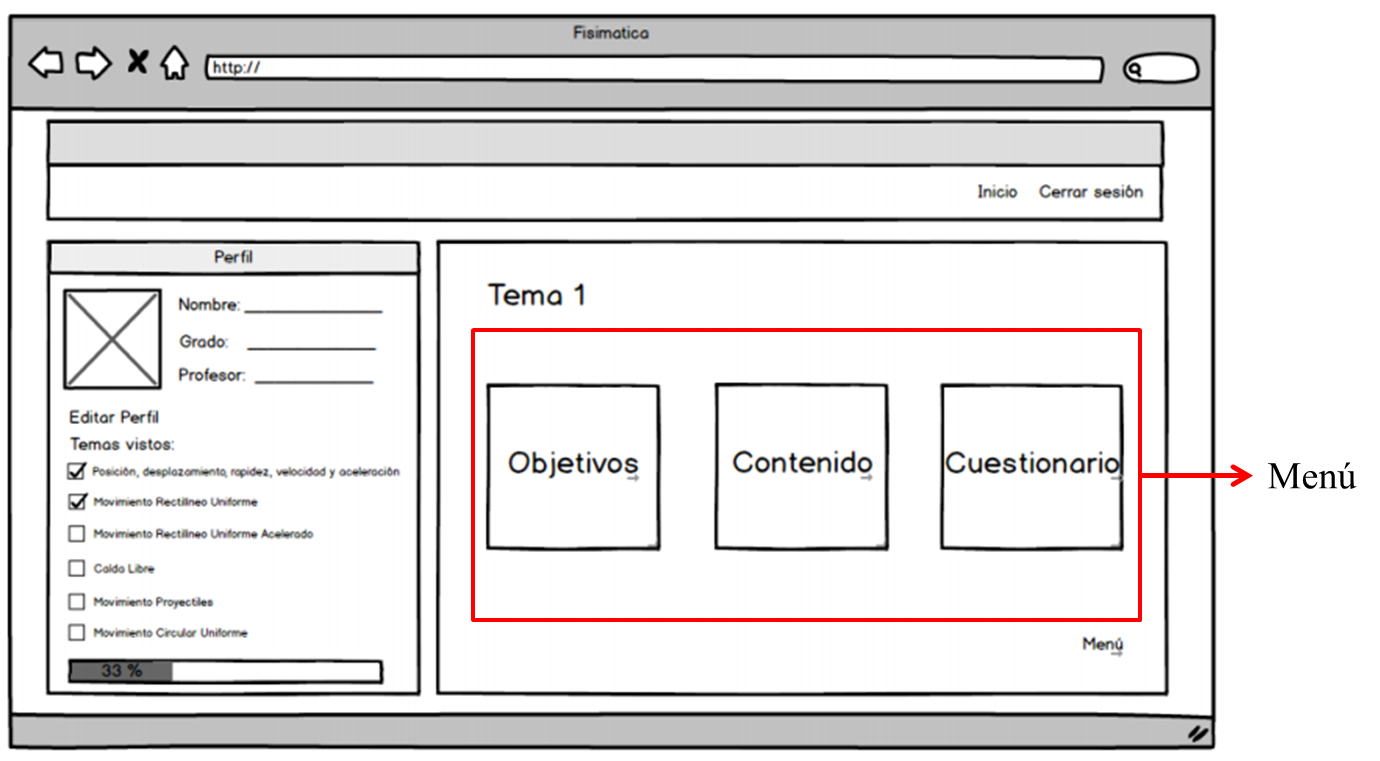
\includegraphics[scale=0.4]{Capitulo_4/2_XP/imagenes/navLibre2.png}
         \caption{Prototipo de navegación Libre - Menú Tema 1}
        \scriptsize \textbf{Fuente:} Elaboración propia
        \label{fig:navLibreMenu}
    \end{figure}

\item \textbf{Categoría Dependiente del Campo}\\
    En el caso de la categoría dependiente del campo, no se ofrece un menú, se ofrece una herramienta de navegación con el fin de ayudar a los alumnos y es el indicador de ``anterior'' y ``siguiente" que hace referencia como su nombre lo indica a visitar la anterior o siguiente página.
    \begin{figure}[H]
    \centering
    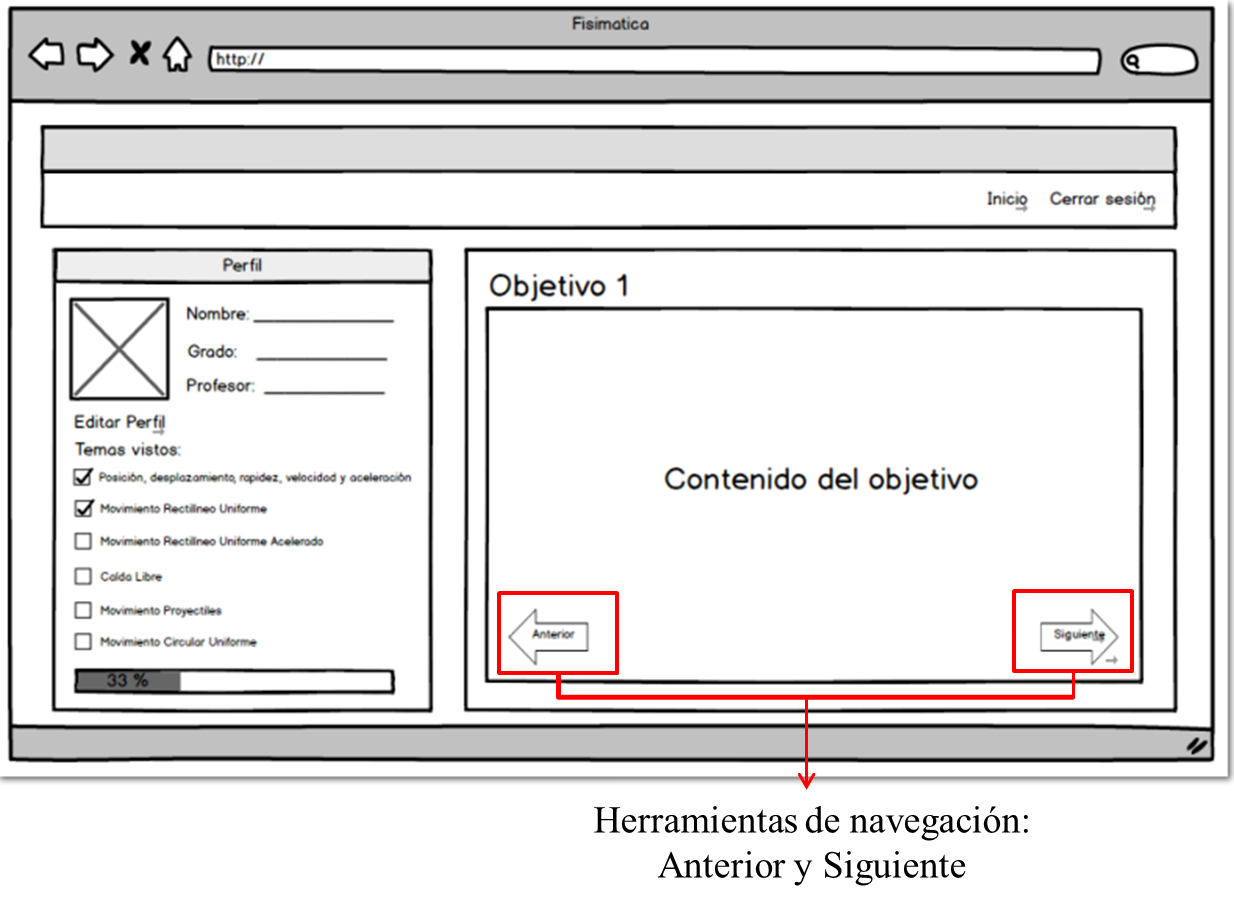
\includegraphics[scale=0.4]{Capitulo_4/2_XP/imagenes/navGuiada.png}
     \caption{Prototipo de la navegación Guiada: Herramienta de navegación (anterior y siguiente)}
    \scriptsize \textbf{Fuente:} Elaboración propia

    \label{fig:navGuia}
\end{figure}

\end{itemize}

\subsubsection{Diagramas de Navegación}

El modelado de la navegación se realizó mediante diagramas, los cuales permitirán representar las actividades de navegación que el estudiante realiza entre el contenido y los elementos de la aplicación; es importante resaltar que existen dos tipos de navegación: Navegación guiada, Navegación libre.

\textbf{Diagrama de navegación libre:}

\begin{figure}[H]
    \centering
    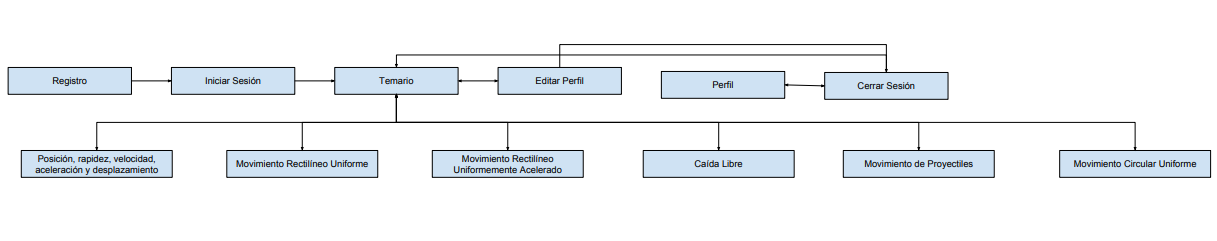
\includegraphics[scale=0.5]{Capitulo_4/2_XP/Navegacion/navegacion1.png}
    \caption{Diagrama navegación libre: Temario}
    \scriptsize \textbf{Fuente: Elaboración propia} 
    \label{fig:navegacionTemario}
\end{figure}

Descripción de las actividades de navegación por parte del estudiante:
\begin{itemize}
    \item Al iniciar sesión el estudiante visualizará el temario, donde este presentará los temas existentes de la cinemática.
    \item Dentro del temario podrá: 
    \begin{itemize}
    \item Desplazarse a la opción de editar perfil y regresar al temario

    \item Desplazarse a la opción perfil para verificar la información que suministro en el registro y regresar al temario
    
    \item Desplazarse al primer módulo denominado Posición, rapidez, velocidad, aceleración y desplazamiento y regresar al temario.
    
    \item Desplazarse al segundo módulo denominado Movimiento Rectilíneo Uniforme y regresar al temario.
    
    \item Desplazarse al tercer módulo denominado Movimiento Rectilíneo y regresar al temario.
    
    \item Desplazarse al cuarto módulo denominado Caída libre y regresar al temario.
    
    \item Desplazarse al quinto módulo denominado Movimiento de Proyectiles y regresar al temario.
    
    \item Desplazarse al sexto módulo denominado Movimiento Circular Uniforme y regresar al temario.
    \end{itemize}
\end{itemize}

 

No obstante  se debe considerar que existen demás escenarios los cuales se han representados de manera individual en
\textbf{(Carpeta Anexos, subcarpeta Diagramas de navegación)}.

\textbf{Diagrama de navegación guiada.}

Se debe considerar que la navegación guiada es meramente establecida por la aplicación de principio a fin, con las opciones de siguiente y anterior, para cambiar de contenido o regresar al contenido en el que el estudiante se encontraba, a continuación, se muestra un ejemplo de un escenario y del diagrama de navegación guiada.

\begin{figure}[H]
    \centering
    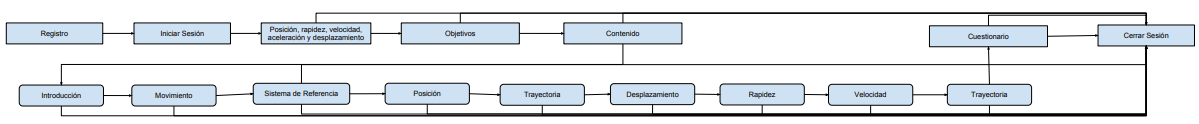
\includegraphics[scale=0.5]{Capitulo_4/2_XP/Navegacion/navegacion2.png}
    \caption{Diagrama navegación guiada: Tema 1}
    \scriptsize \textbf{Fuente: Elaboración propia} 
    \label{fig:navegacionTema1}
\end{figure}








